\chapter{Proposed Method}

The following chapter presents the methodology that will be adopted in the Quantum Retrieval-Augmented Generation (QRAG). QRAG will adopt an architectural approach, whereby it will combine classical methods of retrieval with quantum-based methods of syntactic disambiguation. The primary aim of QRAG is to improve semantic understanding of structural ambiguous queries without compromising efficiency.

\section{Overview of the QRAG Framework}

The QRAG model suggests the development of a hybrid pipeline that is tightly regulated based on the complexity of each query. Instead of using quantum computing for all cases, the algorithm recognizes the patterns of ambiguity and uses quantum processing only when necessary.

The workflow consists of three major stages:
\begin{enumerate}
    \item Ambiguity Detection
    \item Hybrid Processing (Classical or Quantum)
    \item Contextual Realignment and Generation
\end{enumerate}

The overall architecture of the proposed system is illustrated in Figure~\ref{fig:vertical_crag}, which depicts the integration of classical and quantum pipelines within a unified framework.

\begin{figure}[htbp]
    \centering
    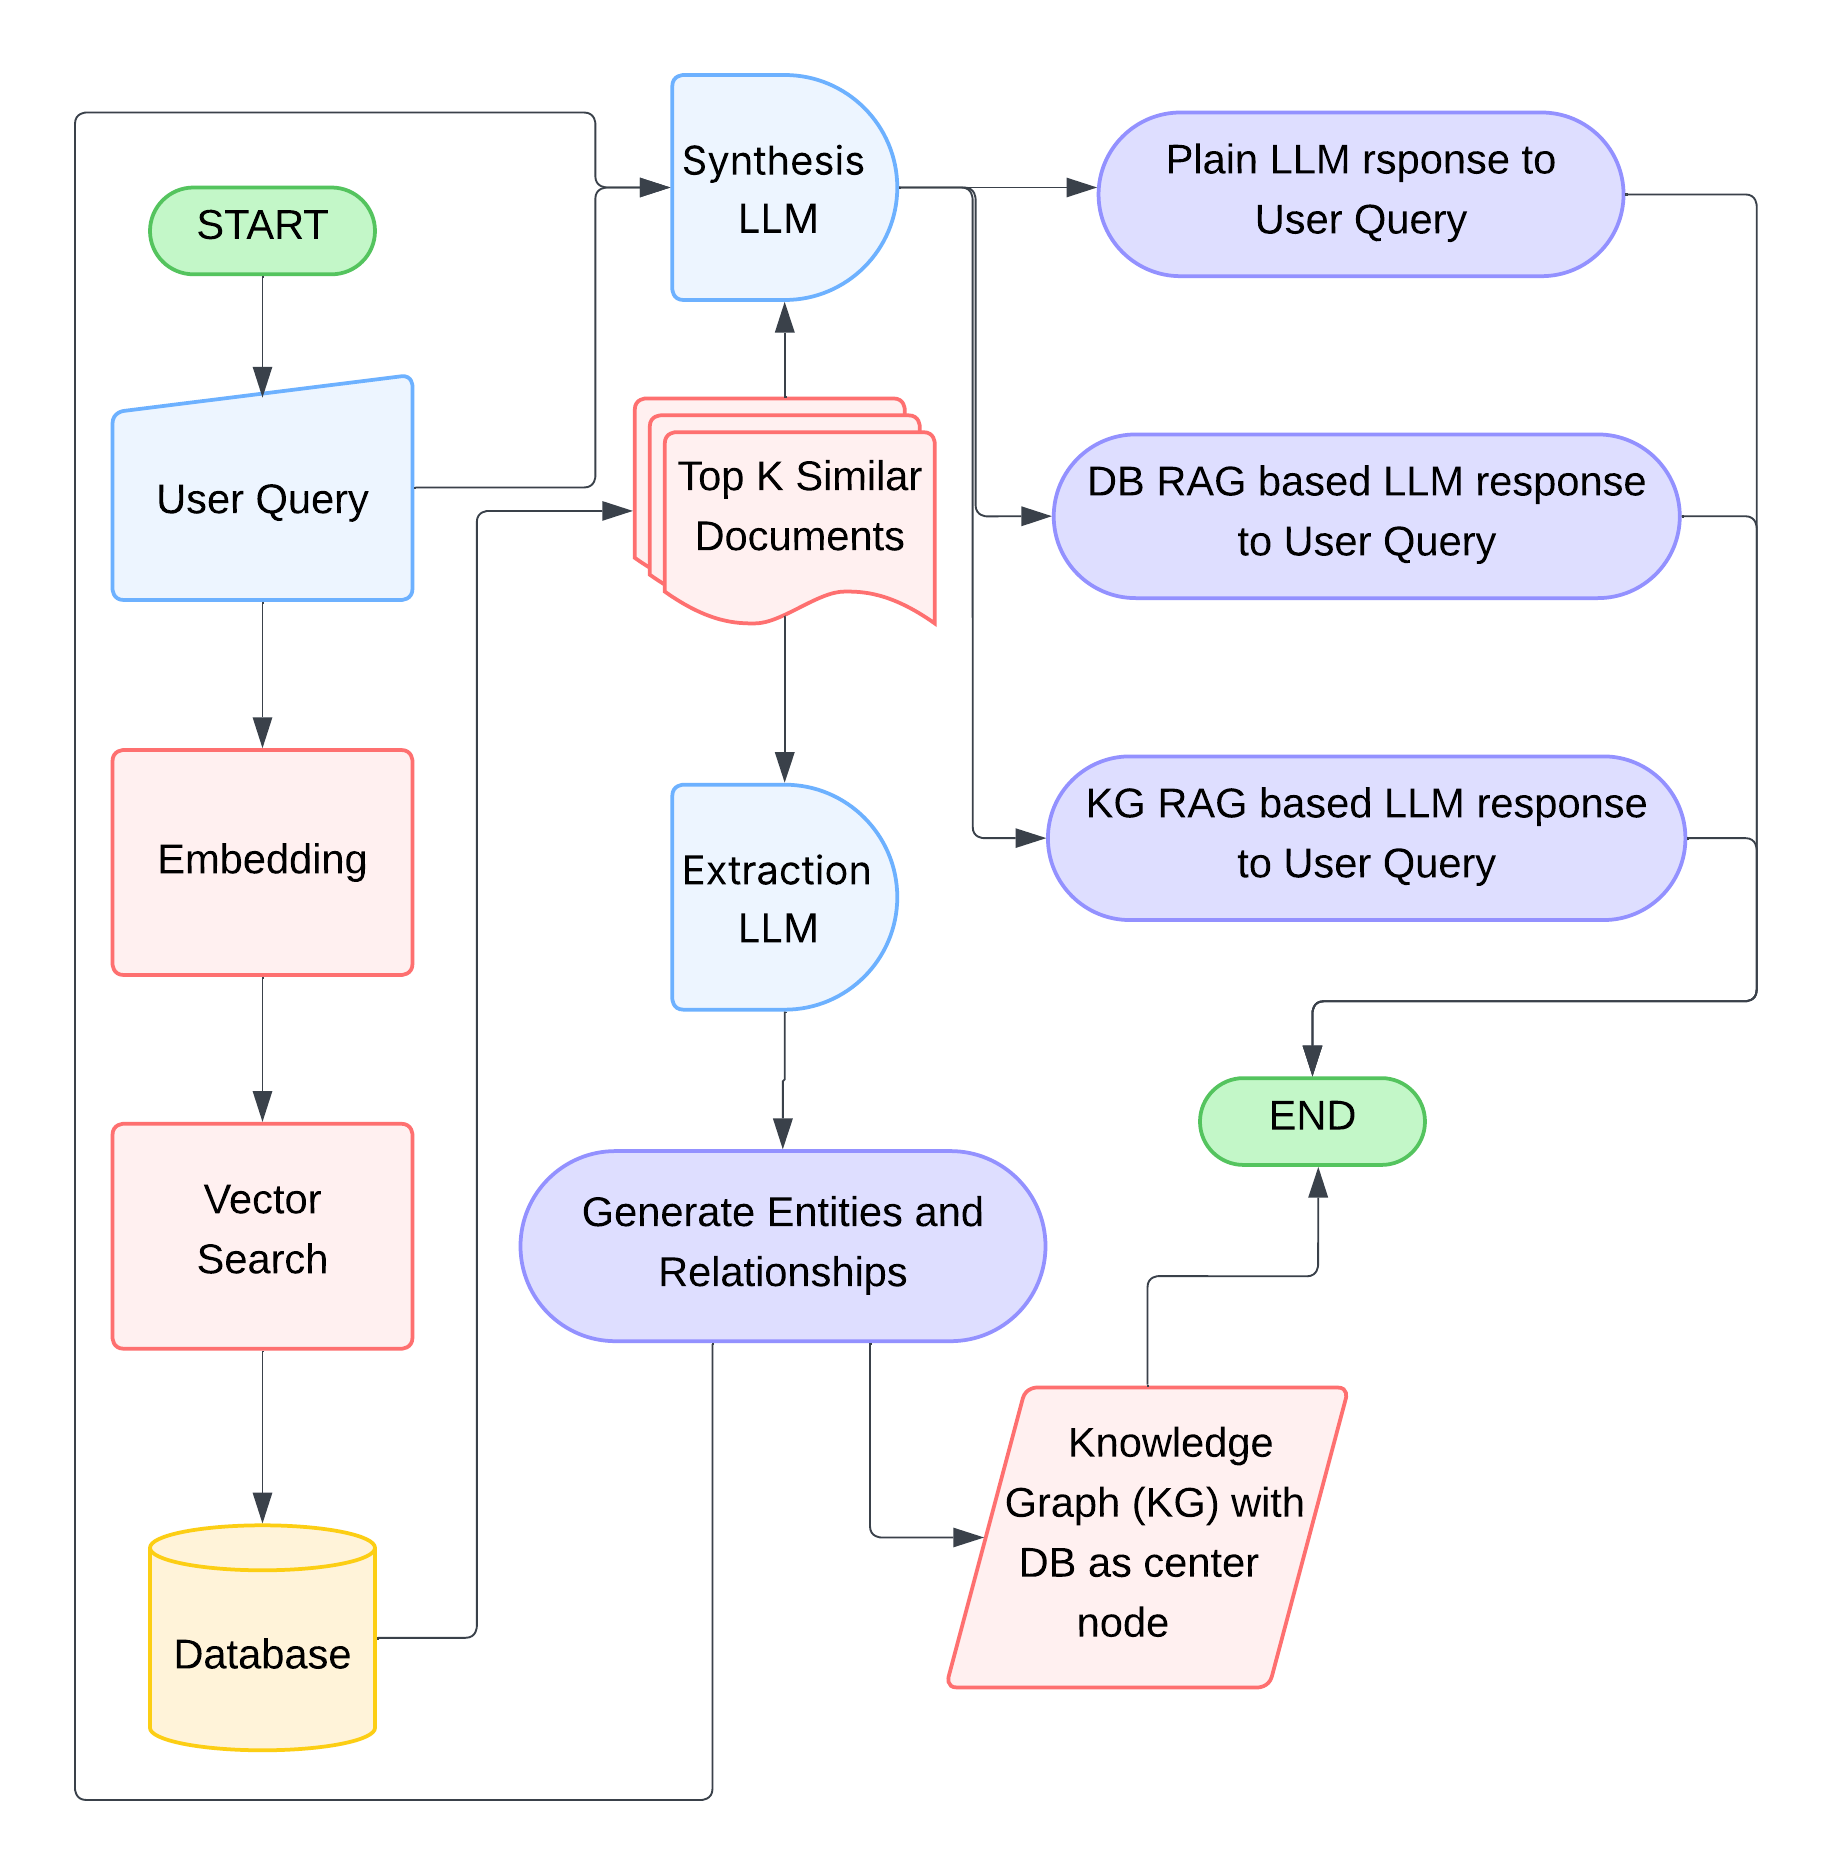
\includegraphics[width=0.85\textwidth]{assets/bnmit/Vertical CRAG Pipeline.png}
    \caption{Vertical CRAG Pipeline diagram illustrating the hybrid processing flow.}
    \label{fig:vertical_crag}
\end{figure}

Additionally, the high-level process flow of ambiguity detection and routing is shown in Figure~\ref{fig:journal_flowchart}.

\begin{figure}[htbp]
    \centering
    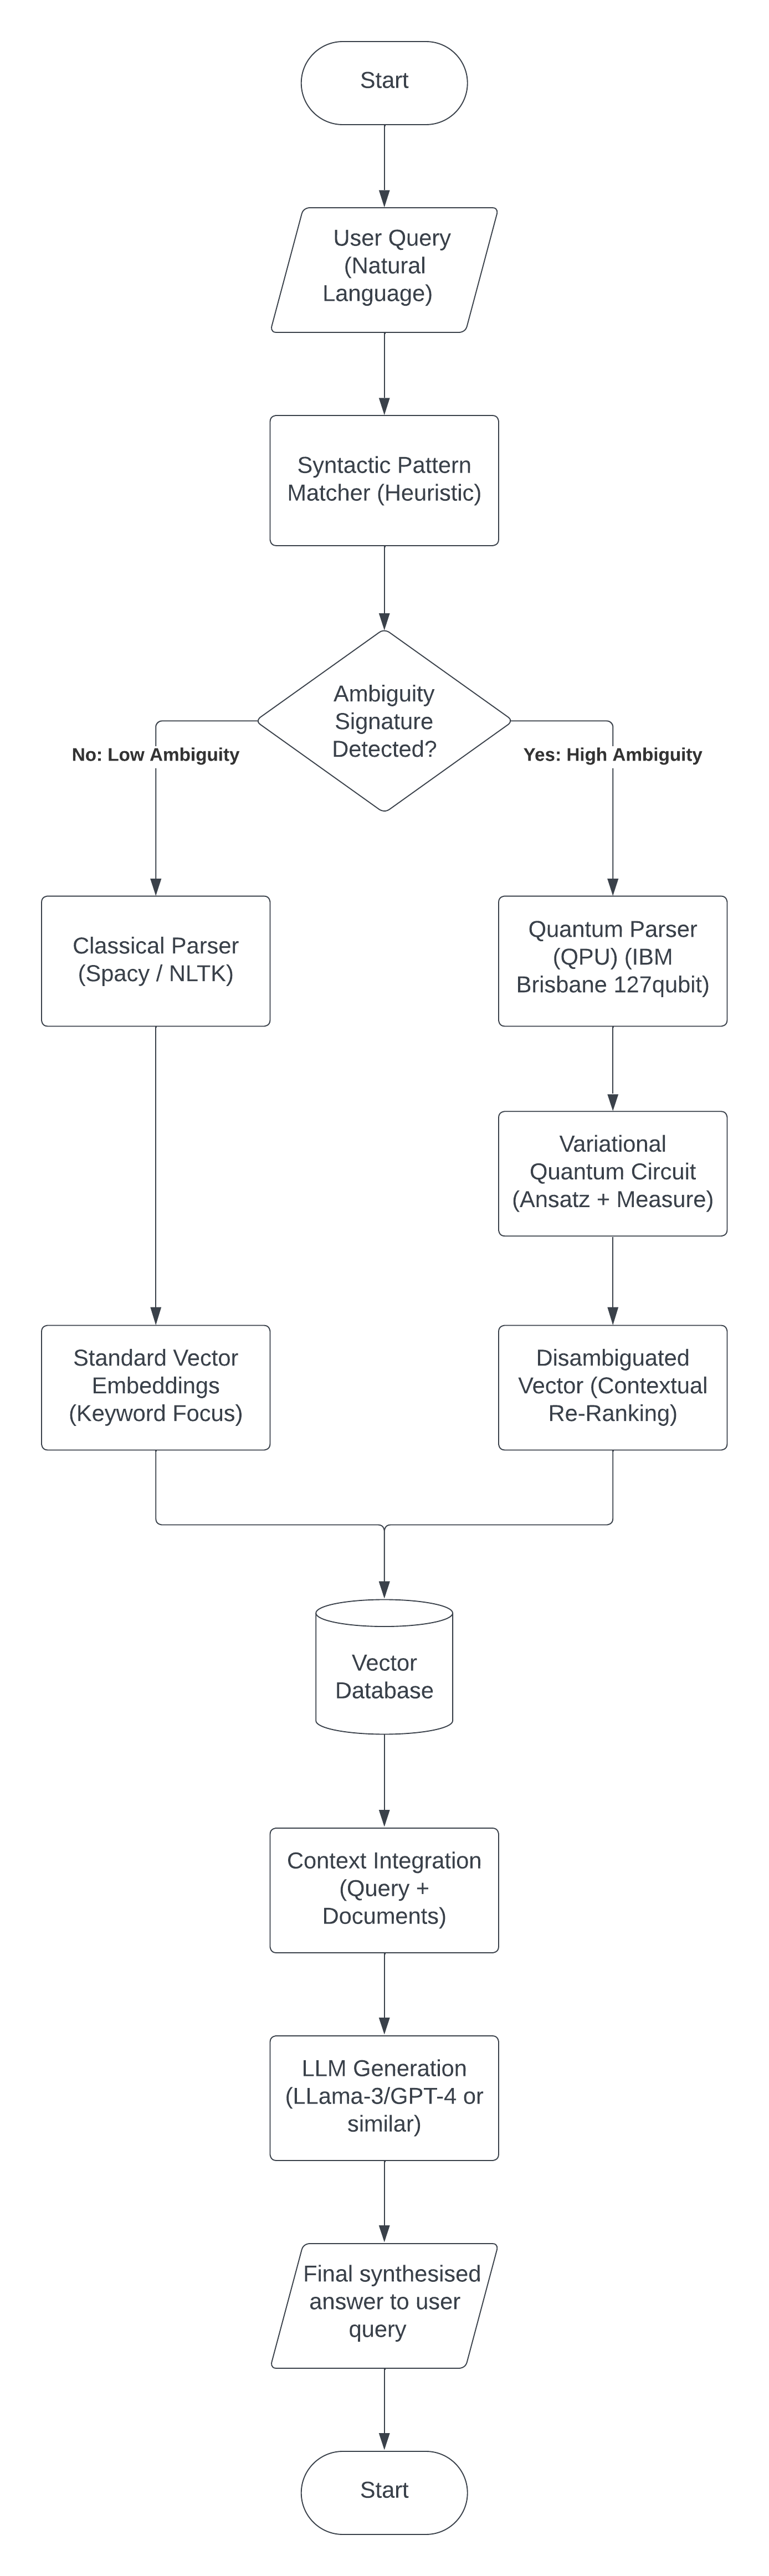
\includegraphics[width=0.4\textwidth]{assets/Journal/flowchart.png}
    \caption{Overall process flowchart of ambiguity detection and routing pipeline.}
    \label{fig:journal_flowchart}
\end{figure}

\section{Ambiguity Detection Mechanism}

The first stage of the process deals with detecting any syntactic ambiguities present in the query. To accomplish this, a simple POS tagging technique is used to analyze the syntax of the query.

The function of ambiguity detection is as follows:

\[
    \delta(q) =
    \begin{cases}
        1, & \text{if } q \text{ contains ambiguity signatures} \\
        0, & \text{otherwise}
    \end{cases}
\]

where $\delta(q)$ determines whether the query should be processed using the quantum pipeline or the classical pipeline.

The system identifies ambiguity using predefined signature patterns such as:
\begin{itemize}
    \item Prepositional Phrase Attachment
    \item Reduced Relative Clauses
    \item Coordination Ambiguity
\end{itemize}

These patterns represent structural configurations where classical parsers are prone to failure.

\section{Hybrid Processing Architecture}

Once ambiguity is detected, the query is routed to one of two processing pipelines.

\subsection{Classical Processing Pipeline}

In the case of simple queries, a classical natural language processing pipeline is used. It involves dependency parsing, vector-based retrieval, and contextual information creation for the process of answer formation. The design of such a pipeline is geared towards ensuring that simple queries will not take long to be processed.

\subsection{Quantum Processing Pipeline}

In cases where the input queries are identified as ambiguous, the quantum pipeline is triggered. In this step, the query is translated to its quantum form through the Variational Quantum Classifier (VQC).

The tokens that make up the input query are mapped to qubits using rotation gates:

\[
    |\psi(x)\rangle = \bigotimes_{i=1}^{N} R_y(\phi(x_i)) |0\rangle_i
\]

Grammatical dependencies between tokens are modeled using Controlled-Z (CZ) entangling gates, enabling the system to capture non-local relationships between words.

The variational quantum circuit is defined as:

\[
    U(\theta) = \prod_{l=1}^{L} \left(U_{ent}^{(l)} \cdot U_{rot}^{(l)}(\theta_l)\right)
\]

The final classification is obtained by measuring the expectation value of an observable, which determines the correct syntactic interpretation.

\section{Contextual Realignment}

The next step after processing is to determine the proper interpretation for the query. This will ensure that the information collected will be in line with the meaning of the query itself.

The interpretation is known as:

\[
    C_{interp} =
    \begin{cases}
        S_1, & \text{if } \hat{y} = 1 \\
        S_0, & \text{otherwise}
    \end{cases}
\]

This refined interpretation is then used to reformulate the query before retrieval and generation.

\section{Integration with Retrieval-Augmented Generation}

After the query disambiguation process, the retrieval stage takes place. Here, relevant documents are identified using semantic similarity from the vector database. The generated context is then fed into the generation model, thereby increasing the accuracy of the facts generated and reducing hallucinations.

\section{Algorithmic Workflow}

The detailed workflow of the proposed method is illustrated in Figure~\ref{fig:cicn_flowchart}. The figure shows the complete sequence from query input to response generation.

\begin{figure}[htbp]
    \centering
    
\includegraphics[width=0.85\textwidth]{assets/cicn/flowchart.png}
    \caption{Detailed algorithmic workflow of the QRAG framework.}
    \label{fig:cicn_flowchart}
\end{figure}

The algorithm can be summarized as follows:

\begin{enumerate}
    \item Accept user query $Q$
    \item Perform preprocessing and POS tagging
    \item Detect syntactic ambiguity
    \item Route query to classical or quantum pipeline
    \item Perform contextual realignment
    \item Retrieve relevant documents
    \item Generate final response using LLM
\end{enumerate}

\section{Design Considerations}

The design of the QRAG framework is guided by the following principles:

\begin{itemize}
    \item \textbf{Efficiency:} Classical processing is used wherever possible to minimize computational overhead.
    \item \textbf{Selective Quantum Usage:} Quantum computation is applied only to complex queries.
    \item \textbf{Modularity:} Independent components improve scalability and maintainability.
    \item \textbf{Extensibility:} The system allows integration of advanced quantum models.
\end{itemize}

\bigskip\noindent
The suggested QRAG model outlines a hybrid approach that takes into consideration the strengths of both classical and quantum computing technologies. In fact, the utilization of ambiguity detection and quantum computation has clearly helped overcome the shortcomings associated with traditional RAG frameworks.
